\documentclass[11pt]{article} \usepackage{fullpage} \usepackage{graphicx} \usepackage{epstopdf} \usepackage{color} \usepackage{psfrag} \usepackage{pdfsync}\usepackage{indentfirst}\usepackage{subfigure}\usepackage{float}\usepackage[section]{placeins}
\usepackage{enumerate}
\usepackage{multirow}
\usepackage{amsfonts, fullpage, graphics} 
\usepackage{algorithm,algorithmic}
\usepackage{amsmath,amssymb,amsthm,bm,hyperref}
\usepackage{dsfont}
\usepackage[parfill]{parskip}
\usepackage[margin=1in]{geometry}
\newcommand{\Lagr}{\mathcal{L}}
\newcommand{\norm}[1]{\left\lVert#1\right\rVert}
\newcommand{\floor}[1]{\lfloor #1 \rfloor}
\newcommand{\todo}[1]{}
\renewcommand{\todo}[1]{{\color{red} TODO: {#1}}}
\newcommand\independent{\protect\mathpalette{\protect\independenT}{\perp}}
\newcommand{\obar}[1]{\mkern 1.5mu\overline{\mkern-1.5mu#1\mkern-1.5mu}\mkern 1.5mu}
\def\independenT#1#2{\mathrel{\rlap{$#1#2$}\mkern2mu{#1#2}}}
\newcommand{\rpm}{\sbox0{$1$}\sbox2{$\scriptstyle\pm$}
  \raise\dimexpr(\ht0-\ht2)/2\relax\box2 }
\usepackage{xspace}
\newcommand{\latex}{\LaTeX\xspace}
\setlength{\parindent}{2em}

\usepackage{listings}
\usepackage{color} %red, green, blue, yellow, cyan, magenta, black, white
\definecolor{mygreen}{RGB}{28,172,0} % color values Red, Green, Blue
\definecolor{mylilas}{RGB}{170,55,241}
\DeclareMathOperator{\E}{\mathbb{E}}
\DeclareMathOperator*{\argmax}{arg\,max}
\DeclareMathOperator*{\argmin}{arg\,min}

\begin{document}

{\parindent 0pt \begin{tabular}[t]{l} 16-720 Computer Vision \\ Spring 2020 \end{tabular}}%  \hfill XX/XX/14 \vskip 0.2in }
\parindent 0pt \parskip 8pt
\begin{center} \large\bf Homework 3 \end{center}
\begin{center} \large\bf Zongwen Mu, Andrew ID: zongwenm \end{center}
\bigskip


\section{Lucas-Kanade Tracking}

\setlength{\parindent}{2em}  

\paragraph{Q1.1}~{}

For a warp function:
\begin{align}
	\mathcal{W}\left(\bold{x}; \bold{p}\right) & = 
	\begin{bmatrix}
	\mathcal{W}_x \\
	\mathcal{W}_y
	\end{bmatrix}
	= \begin{bmatrix}
	1 & 0 & p_1 \\
	0 & 1 & p_2
	\end{bmatrix}
	\begin{bmatrix}
	x \\ y \\ 1
	\end{bmatrix} \\
	& = \begin{bmatrix}
	x + p_1 \\ y + p_2
	\end{bmatrix}
\end{align}

Therefore:
\begin{align}
	\frac{\partial{\mathcal{W}\left(\bold{x}; \bold{p}\right)}}{\partial{\bold{p}^{T}}} & =
	\begin{bmatrix}
		\frac{\partial{\mathcal{W}_{x}\left(\bold{x}, \bold{p}\right)}}{\partial{\bold{p}_{1}^{T}}} & \frac{\partial{\mathcal{W}_{x}\left(\bold{x}, \bold{p}\right)}}{\partial{\bold{p}_{2}^{T}}} \\
		\frac{\partial{\mathcal{W}_{y}\left(\bold{x}, \bold{p}\right)}}{\partial{\bold{p}_{1}^{T}}} & \frac{\partial{\mathcal{W}_{y}\left(\bold{x}, \bold{p}\right)}}{\partial{\bold{p}_{2}^{T}}}	
	\end{bmatrix} \\
	& =
	\begin{bmatrix}
		1 & 0 \\
		0 & 1
	\end{bmatrix}
\end{align}

Since we are trying to obtain:
\begin{align}
	& \mathop{\arg\min}_{\Delta{p}} \sum_{\mathbf{x} \in \mathbb{N}} \left \| \mathcal{I}_{t+1}\left( \mathbf{x^\prime} + \Delta{\mathbf{p}} \right) - \mathcal{I}_{t}\left( \mathbf{x} \right) \right \|_{2}^{2} \\
	& = \mathop{\arg\min}_{\Delta{p}} \sum_{\mathbf{x} \in \mathbb{N}} \left \| \mathcal{I}_{t+1}\left( \mathbf{x^\prime} \right) + \frac{\partial{\mathcal{I}_{t+1}\left( \mathbf{x^\prime} \right)}}{\partial{\bold{x^\prime}^{T}}}\frac{\partial{\mathcal{W}\left(\bold{x}; \bold{p}\right)}}{\partial{\bold{p}^{T}}}\Delta{\mathbf{p}} - \mathcal{I}_{t}\left( \mathbf{x} \right) \right \|_{2}^{2} \\
	& = \mathop{\arg\min}_{\Delta{p}} \sum_{\mathbf{x} \in \mathbb{N}} \left \| \frac{\partial{\mathcal{I}_{t+1}\left( \mathbf{x^\prime} \right)}}{\partial{\bold{x^\prime}^{T}}}\frac{\partial{\mathcal{W}\left(\bold{x}; \bold{p}\right)}}{\partial{\bold{p}^{T}}}\Delta{\mathbf{p}} - \left[\mathcal{I}_{t}\left( \mathbf{x} \right) - \mathcal{I}_{t+1}\left( \mathbf{x^\prime} \right) \right] \right \|_{2}^{2}
\end{align}

Where $\bold{x^\prime} = \bold{x} + \bold{p}$.

Therefore, we have:
\begin{align}
	\mathbf{A} & = \frac{\partial{\mathcal{I}_{t+1}\left( \mathbf{x^\prime} \right)}}{\partial{\bold{x^\prime}^{T}}}\frac{\partial{\mathcal{W}\left(\bold{x}; \bold{p}\right)}}{\partial{\bold{p}^{T}}} \\
	& = \begin{bmatrix}
	\frac{\partial{\mathcal{I}_{t+1}\left( \mathbf{x_{1}^\prime} \right)}}{\partial{\bold{x_{1}^\prime}^{T}}} & \cdots & 0 \\
	\vdots & \ddots & \vdots \\
	0 & \cdots & \frac{\partial{\mathcal{I}_{t+1}\left( \mathbf{x_{D}^\prime} \right)}}{\partial{\bold{x_{D}^\prime}^{T}}}
	\end{bmatrix} \begin{bmatrix}
	\frac{\partial{\mathcal{W}\left(\bold{x_1}; \bold{p}\right)}}{\partial{\bold{p}^{T}}} \\ \vdots \\ \frac{\partial{\mathcal{W}\left(\bold{x_D}; \bold{p}\right)}}{\partial{\bold{p}^{T}}}
	\end{bmatrix}
\end{align}
\begin{align}
	\mathbf{b} & = \mathcal{I}_{t}\left( \mathbf{x} \right) - \mathcal{I}_{t+1}\left( \mathbf{x^\prime} \right) \\
	& = \begin{bmatrix}
	\mathcal{I}_{t}\left( \mathbf{x_1} \right) - \mathcal{I}_{t+1}\left( \mathbf{x_1^\prime} \right) \\ \vdots \\ \mathcal{I}_{t}\left( \mathbf{x_D} \right) - \mathcal{I}_{t+1}\left( \mathbf{x_D^\prime} \right)
	\end{bmatrix}
\end{align}

To guarantee a unique solution for $\Delta\mathbf{p}$, $\mathbf{A^TA}$ needs to be full rank, in other words, $det\left(\mathbf{A^TA} \right) \ne 0$

\paragraph{Q1.3}~{}

Result pictures are shown below:
\begin{figure}[H]
\centering
\subfigure[]{
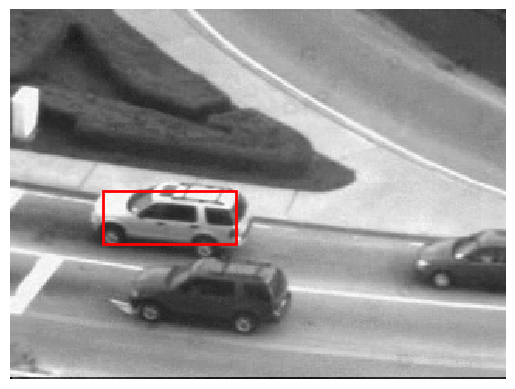
\includegraphics[width=0.15\textwidth]{results/carseq1.png}}
\subfigure[]{
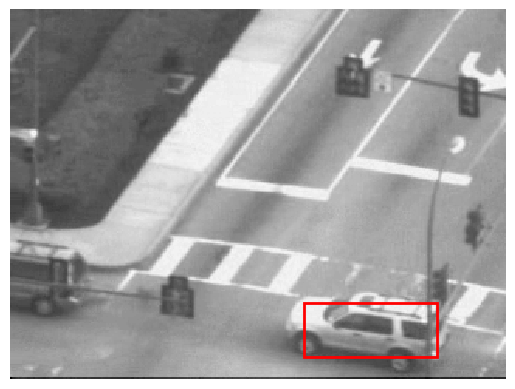
\includegraphics[width=0.15\textwidth]{results/carseq100.png}}
\subfigure[]{
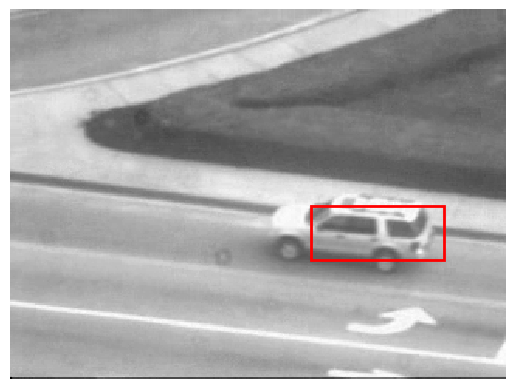
\includegraphics[width=0.15\textwidth]{results/carseq200.png}}
\subfigure[]{
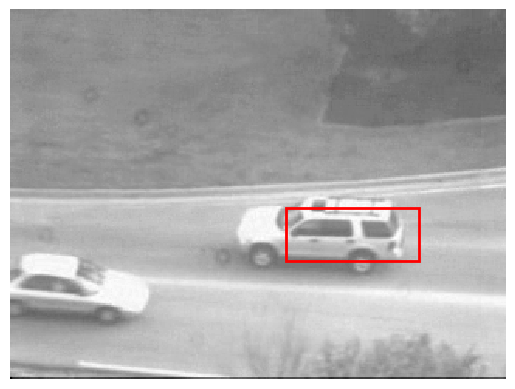
\includegraphics[width=0.15\textwidth]{results/carseq300.png}}
\subfigure[]{
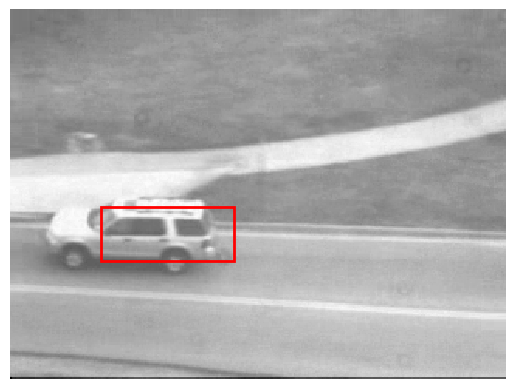
\includegraphics[width=0.15\textwidth]{results/carseq400.png}}
\caption{Car Sequence with One Single Template}
\end{figure}

\begin{figure}[H]
\centering
\subfigure[]{
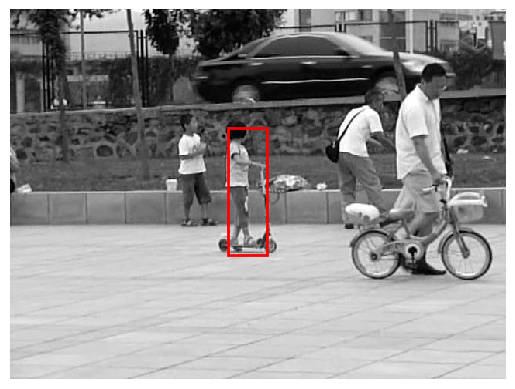
\includegraphics[width=0.15\textwidth]{results/girlseq1.png}}
\subfigure[]{
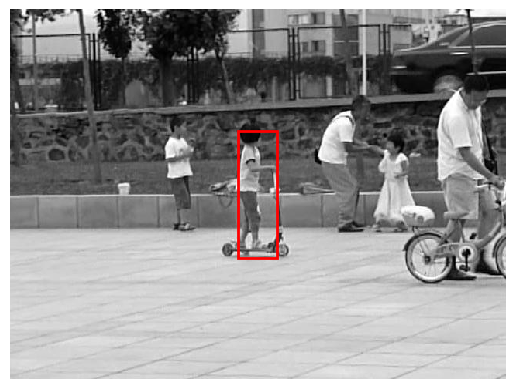
\includegraphics[width=0.15\textwidth]{results/girlseq20.png}}
\subfigure[]{
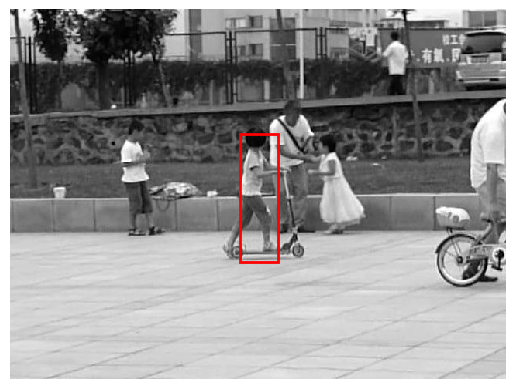
\includegraphics[width=0.15\textwidth]{results/girlseq40.png}}
\subfigure[]{
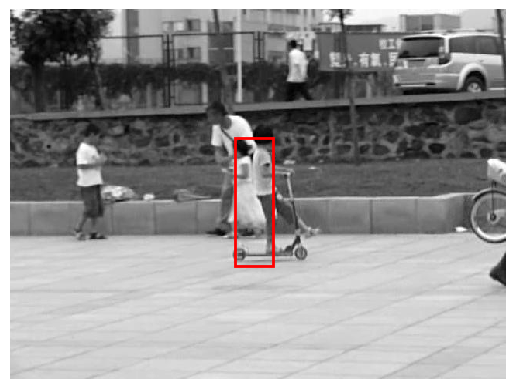
\includegraphics[width=0.15\textwidth]{results/girlseq60.png}}
\subfigure[]{
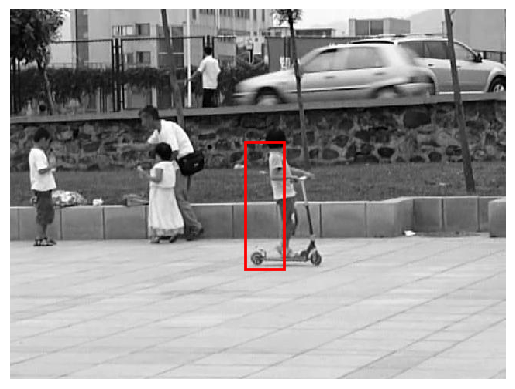
\includegraphics[width=0.15\textwidth]{results/girlseq80.png}}
\caption{Girl Sequence with One Single Template}
\end{figure}

\paragraph{Q1.4}~{}

Result pictures are shown below, in which red rectangles are created by baseline tracker with correction and blue rectangles are those created in $\bold{Q1.3}$:
\begin{figure}[H]
\centering
\subfigure[]{
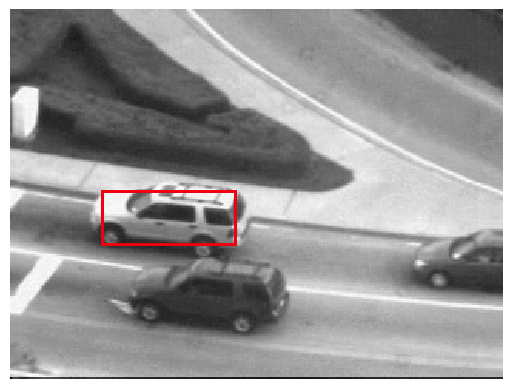
\includegraphics[width=0.15\textwidth]{results/carseq_wrct1.png}}
\subfigure[]{
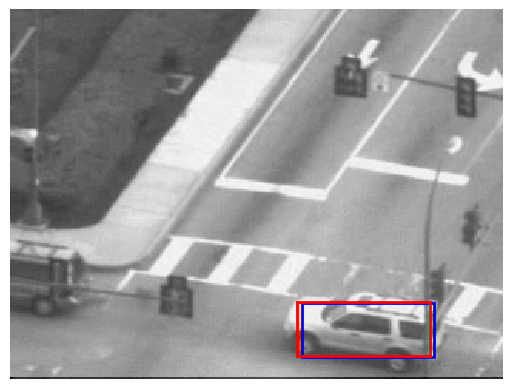
\includegraphics[width=0.15\textwidth]{results/carseq_wrct100.png}}
\subfigure[]{
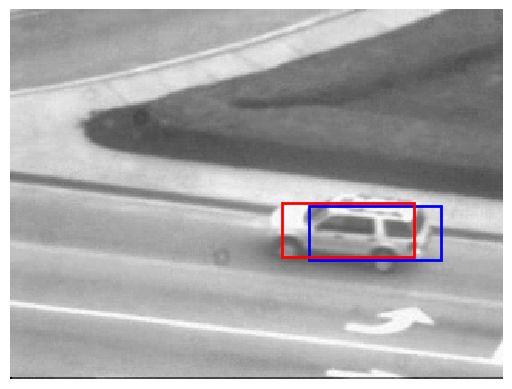
\includegraphics[width=0.15\textwidth]{results/carseq_wrct200.png}}
\subfigure[]{
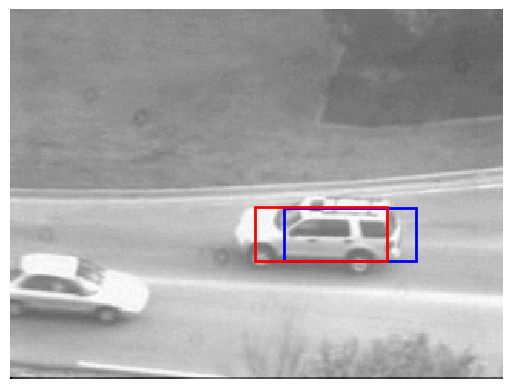
\includegraphics[width=0.15\textwidth]{results/carseq_wrct300.png}}
\subfigure[]{
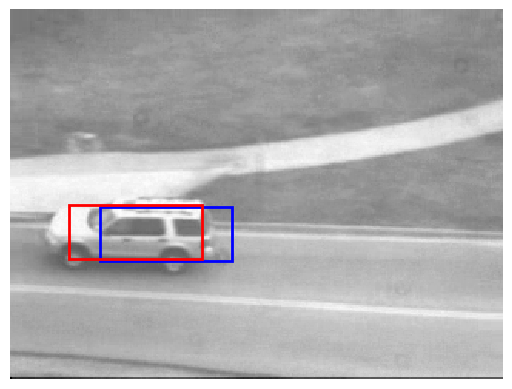
\includegraphics[width=0.15\textwidth]{results/carseq_wrct400.png}}
\caption{Car Sequence with Template Correction}
\end{figure}

\begin{figure}[H]
\centering
\subfigure[]{
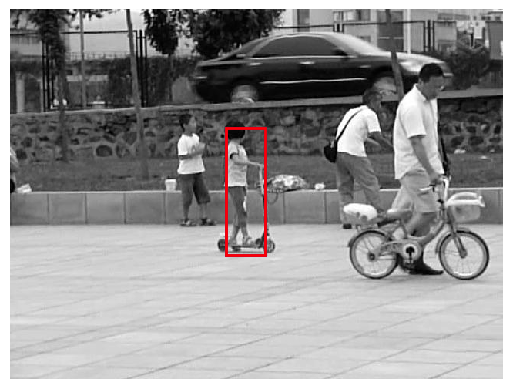
\includegraphics[width=0.15\textwidth]{results/girlseq_wrct1.png}}
\subfigure[]{
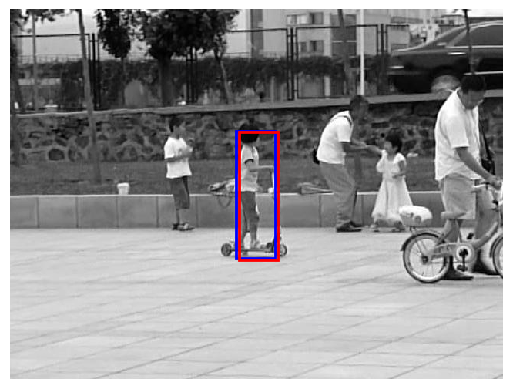
\includegraphics[width=0.15\textwidth]{results/girlseq_wrct20.png}}
\subfigure[]{
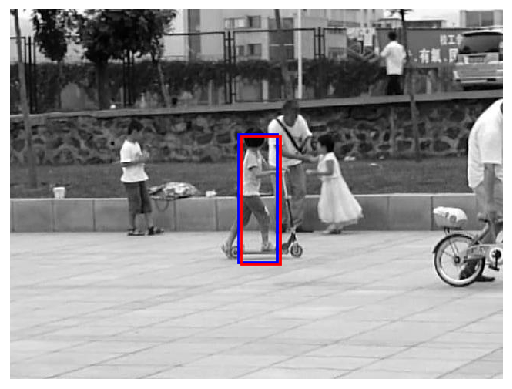
\includegraphics[width=0.15\textwidth]{results/girlseq_wrct40.png}}
\subfigure[]{
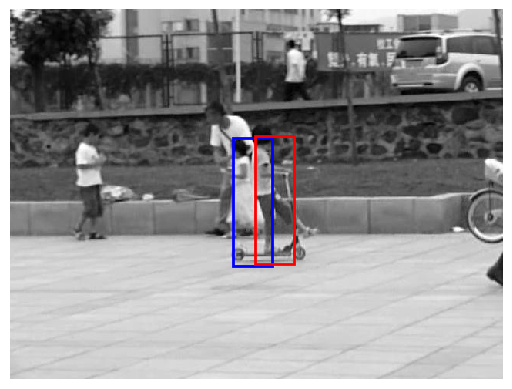
\includegraphics[width=0.15\textwidth]{results/girlseq_wrct60.png}}
\subfigure[]{
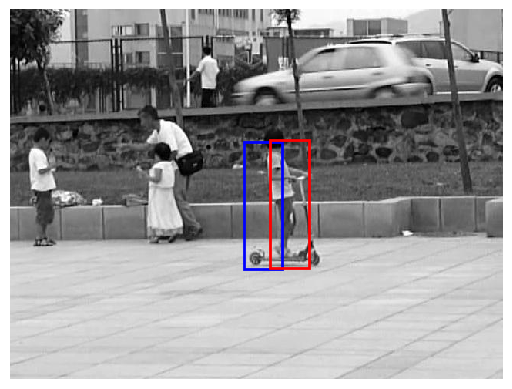
\includegraphics[width=0.15\textwidth]{results/girlseq_wrct80.png}}
\caption{Girl Sequence with Template Correction}
\end{figure}

\section{Affine Motion Subtraction}

\paragraph{Q2.3}~{}

Result images are shown below:
\begin{figure}[H]
\centering
\subfigure[]{
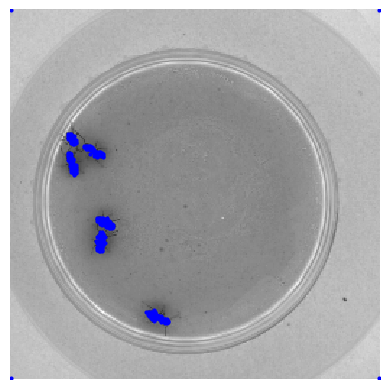
\includegraphics[width=0.2\textwidth]{results/antseq30.png}}
\subfigure[]{
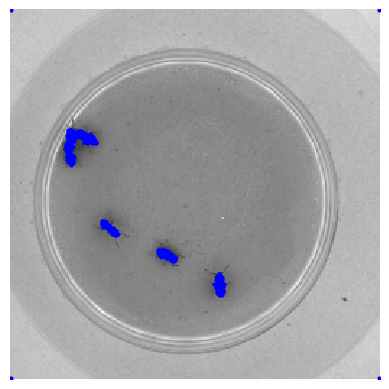
\includegraphics[width=0.2\textwidth]{results/antseq60.png}}
\subfigure[]{
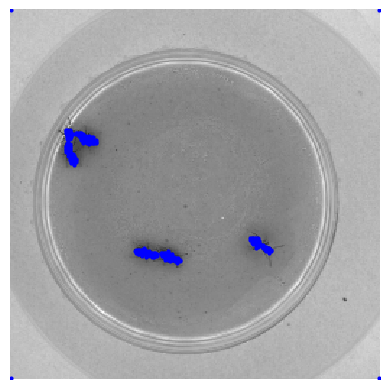
\includegraphics[width=0.2\textwidth]{results/antseq90.png}}
\subfigure[]{
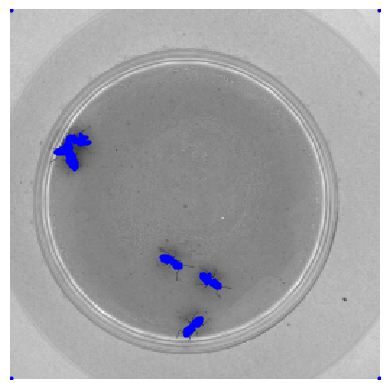
\includegraphics[width=0.2\textwidth]{results/antseq120.png}}
\caption{Motion Detection of Ant Sequence}
\end{figure}

\begin{figure}[H]
\centering
\subfigure[]{
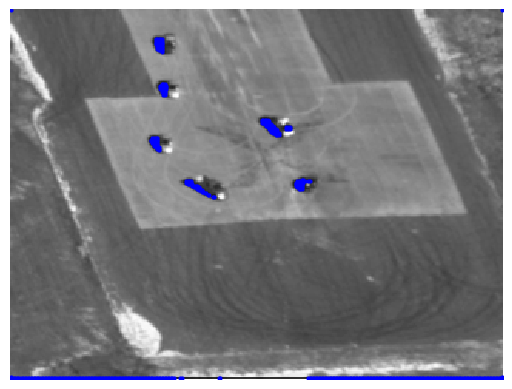
\includegraphics[width=0.2\textwidth]{results/aerialseq30.png}}
\subfigure[]{
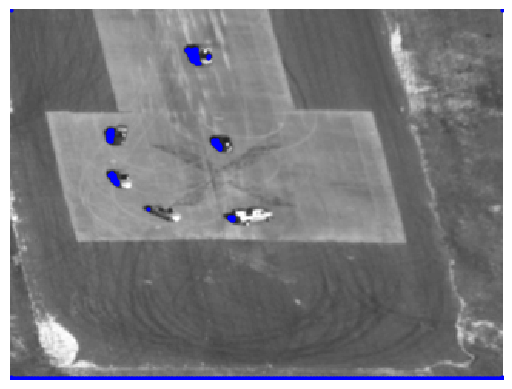
\includegraphics[width=0.2\textwidth]{results/aerialseq60.png}}
\subfigure[]{
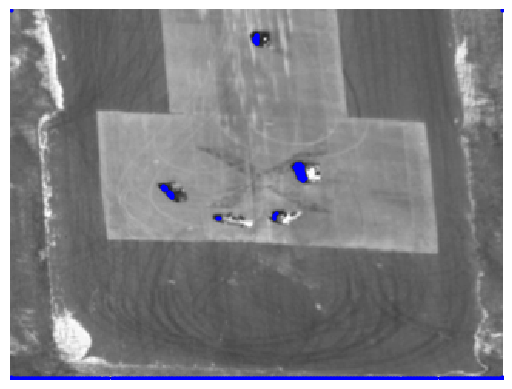
\includegraphics[width=0.2\textwidth]{results/aerialseq90.png}}
\subfigure[]{
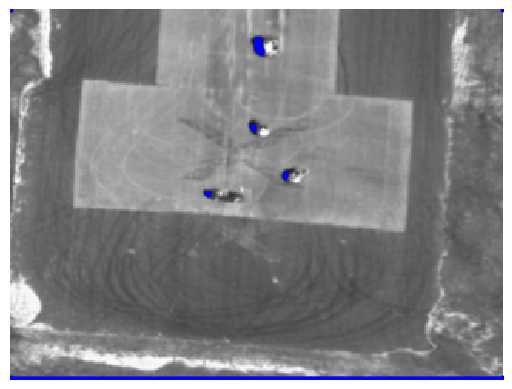
\includegraphics[width=0.2\textwidth]{results/aerialseq120.png}}
\caption{Motion Detection of Aerial Sequence}
\end{figure}

\section{Efficient Tracking}

\paragraph{Q3.1}~{}

Because some time-consuming tasks like Hessian, steepest descent images could be pre-computed, so we do not need to compute it repeatedly in optimization gradient descent iterations.

\end{document}
